% SPDX-FileCopyrightText: 2023 SAP SE
%
% SPDX-License-Identifier: Apache-2.0
%
% This file is part of FEDEM - https://openfedem.org

%%%%%%%%%%%%%%%%%%%%%%%%%%%%%%%%%%%%%%%%%%%%%%%%%%%%%%%%%%%%%%%%%%%%%%%%%%%%%%%%
%
% FEDEM User Guide.
%
%%%%%%%%%%%%%%%%%%%%%%%%%%%%%%%%%%%%%%%%%%%%%%%%%%%%%%%%%%%%%%%%%%%%%%%%%%%%%%%%

\Chapter{Wind Power Modeling}{wind-power-modeling}

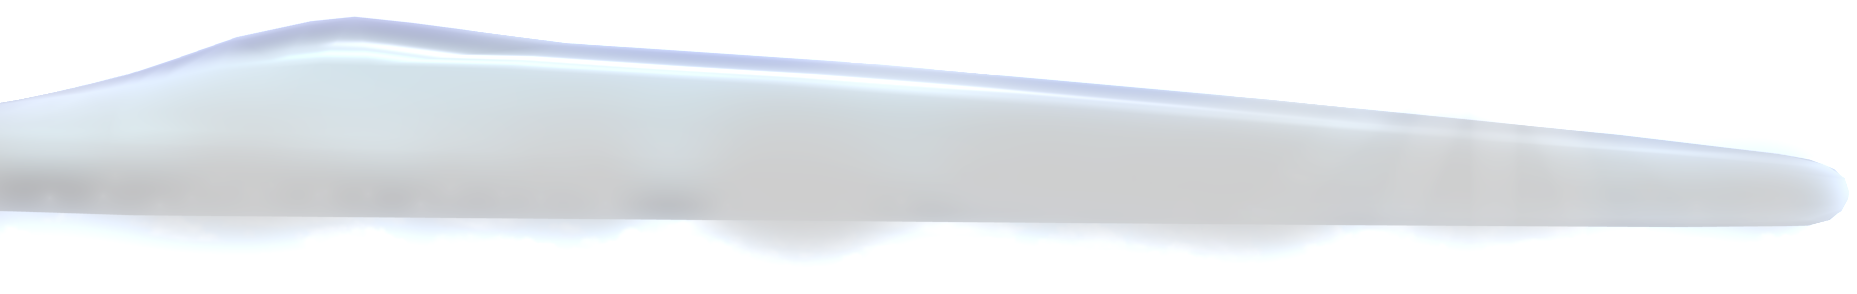
\includegraphics[width=\textwidth]{Figures/3b-Head1}

This chapter describes how to perform the basic operations you need to do,
in order to build wind turbine models, such as defining the turbine,
defining the tower, adjusting the model, etc.

The wind power features of Fedem (which in the following are referred to as
{\sl Fedem Windpower}) use the {\sl AeroDyn} module of the
National Renewable Energy Laboratory (NREL) in the USA
(\href{https://wind.nrel.gov/}{wind.nrel.gov}), for all calculations related to
the aerodynamic loads on the wind turbine blades. These loads are then applied
onto the structural model of the wind turbine in the Fedem dynamics solver,
to provide response data that can be further analysed.

The basic mechanism elements of Fedem (parts, triads, joints, etc.) and their
properties are discussed in detail in
\refChapter{mechanism-elements}{Mechanism Elements}.
This chapter focuses on issues specific to wind turbine modeling only.

Sections in this chapter address the following topics:

\begin{itemize}
%\item
%  \protect\hyperlink{wind-turbine-modeling-approaches}
%                    {Wind turbine modeling approaches}
\item
  \protect\hyperlink{creating-a-basic-wind-turbine-model}
                    {Creating a basic wind turbine model}
\item
  \protect\hyperlink{basic-solving-and-analysis}
                    {Basic solving and analysis}
\item
  \protect\hyperlink{creating-an-advanced-wind-turbine-model}
                    {Creating an advanced wind turbine model}
\item
  \protect\hyperlink{advanced-solving-and-analysis}
                    {Advanced solving and analysis}
\end{itemize}

\clearpage

%Think we skip this section on (other) modeling approaches.
%% SPDX-FileCopyrightText: 2023 SAP SE
%
% SPDX-License-Identifier: Apache-2.0
%
% This file is part of FEDEM - https://openfedem.org

\Section{Wind turbine modeling approaches}{wind-turbine-modeling-approaches}

There are alternative approaches to wind turbine modeling:

\begin{itemize}
\item{\sl NREL/FAST} --
  The FAST software is the first generation of wind turbine modeling tools.
  The software is developed as a part of a public research project at
  the National Renewable Energy Laboratory.
  The FAST software is open source, which is important in many research projects
  that seek to advance scientific knowledge within the area.
  The tool does, however, not have a graphical user interface and can be
  difficult to use correctly in a fast-pased commercial application.
\item{\sl GLGH/Bladed} --
  The Bladed software is the first generation of privately developed and
  commercially available wind turbine modeling tools.
  The tool basically adds a graphical user interface to the wind
  turbine modeling process. A set of dialog boxes are used to input
  options and data. The tool offers a straight-forward approach to the
  wind turbine modeling process that works well for typical wind turbine models.
\item{\sl Fedem WindPower} --
  We, respectfully, offer Fedem WindPower as a next generation wind turbine
  modeling environment. The Fedem software is designed and developed to be
  a high-end technology platform and an engineering framework for virtual
  testing of complex mechanical assemblies. It provides a complete set of
  features to create, solve and post-process wind turbine models in a
  3D graphical environment.
  We can offer our software as a complete replacement of prior software.
\end{itemize}

There are additional wind turbine modeling tools as well that are made
at universities, research institutions and elsewhere but they are in the
design line of first generation tools, for the most part.

Fedem WindPower is the only software that offers a high-end technology platform
and engineering framework for virtual testing of complex wind turbine models.
Fedem WindPower includes a large array of mechanism elements such as parts,
joints, springs, dampers, loads, control systems, and so on,
that can be added to (or modified in) the wind turbine model.
Each mechanism element has a large array of properties that offers fine detail
control over the model. The solvers produce results that offer an easy and
intuitive analysis approach with integrated graphs and tables.
Results can also be exported to other tools.
Never before have wind turbine modeling, solving and analysis been this easy,
flexible, extensible, comprehensible, precise, auditable and powerful!


%%%%%%%%%%%%%%%%%%%%%%%%%%%%%%%%%%%%%%%%%%%%%%%%%%%%%%%%%%%%%%%%%%%%%%%%%%%%%%%%
\Section{Creating a basic wind turbine model}
        {creating-a-basic-wind-turbine-model}

The Fedem Windpower user interface is illustrated in the figure below.
Here we see the start up screen when you have just launched the application.

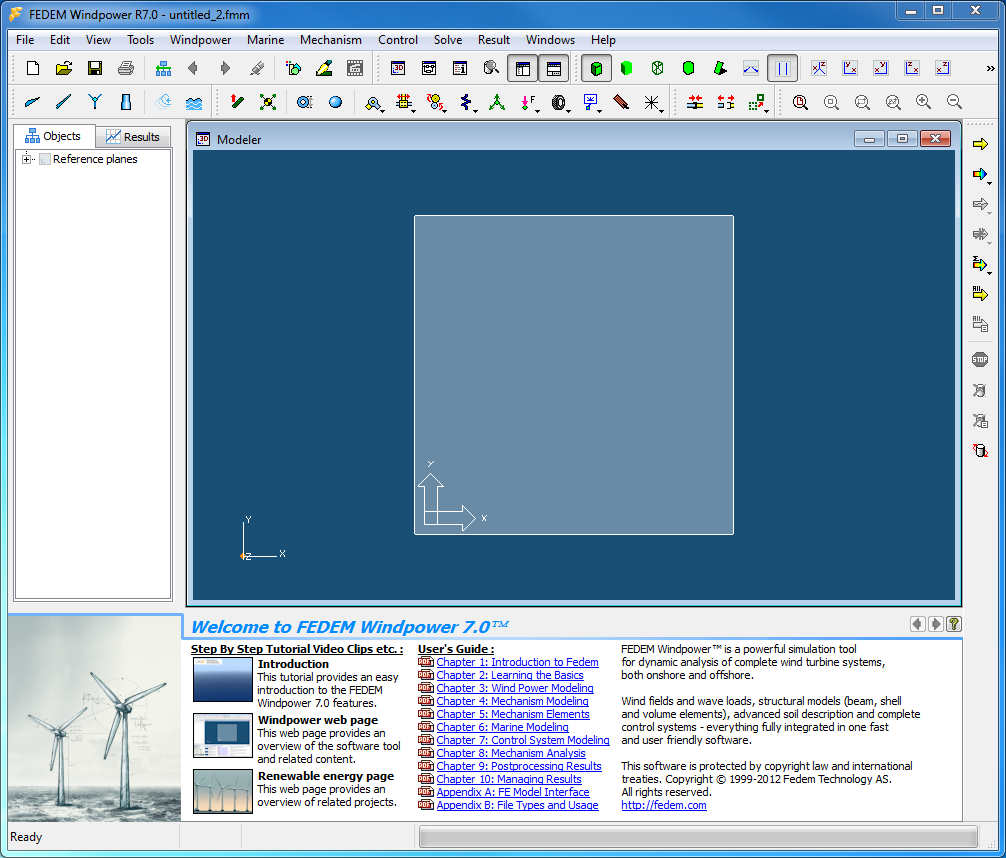
\includegraphics[width=0.9\textwidth]{Figures/3b-Main1}

Fedem Windpower has a few major additional features,
as compared to the standard edition:

\subsubsection{Windpower menu}

\begin{wrapfigure}[9]{r}{0.35\textwidth}
  \vskip-2\baselineskip
  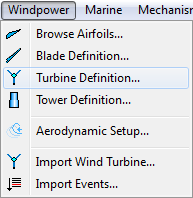
\includegraphics[width=0.35\textwidth]{Figures/3b-WindpowerMenu}
\end{wrapfigure}

The main window includes the {\sl Windpower} menu \newline
(shown at right). It contains choices for creating \newline
and updating the wind turbine model, \newline
for aerodynamic setup, etc.

The \textbf{Import Wind Turbine...} entry \newline
provides an alternative (obsolescent) way of \newline
specifying a turbine setup. It is present for \newline
backward compatibility only and should not \newline
be used when starting a new project.

The \textbf{Import Events...} entry is used for setting up simulation events,
which is handy when you have a large simulation setup with many load cases on
an (almost) identical structural model.
Refer to \refSection{using-simulation-events}{Using simulation events} for
learning more on how to set up and use simulation events.

\subsubsection{Marine menu}

\begin{wrapfigure}[10]{r}{0.35\textwidth}
  \vskip-1.2\baselineskip
  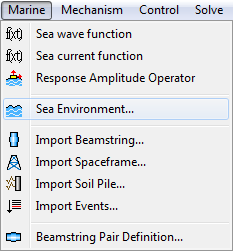
\includegraphics[width=0.35\textwidth]{Figures/3b-MarineMenu}
\end{wrapfigure}

The main window also includes the {\sl Marine} menu (shown at right).
It contains choices for defining the marine environment when modeling an
offshore wind turbine.
Refer to \refChapter{marine-modeling}{Marine Modeling}
for full details on these items.
The {\sl Marine} menu also contains entries for importing higher-level
structural components that are subjected to marine loads, such as space frames
(Jackets), soil piles and general beam strings.
It also contains the same \textbf{Import Events...} entry
as in the {\sl Windpower} menu.

\subsubsection{Windpower tool bar}

\begin{wrapfigure}[2]{r}{0.3\textwidth}
  \vskip-\baselineskip
  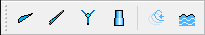
\includegraphics[width=0.3\textwidth]{Figures/3b-WindpowerToolbar}
\end{wrapfigure}

The {\sl Windpower} tool bar (shown at right) provides an easy access to
the mostly used choices of the {\sl Windpower} and {\sl Marine} menus,
when modeling offshore wind turbines.

\clearpage


\SubSection{Turbine definition}{turbine-definition}

Fedem Windpower provides a set of dialog boxes for creating wind turbine models.
Let us first have a look at the Turbine Definition dialog box.

\IconText{turbineDef}{To open the
Turbine Definition dialog box, click the \textbf{Turbine Definition...} button
on the menu or tool bar. The Turbine Definition dialog box is shown below
with the default turbine assembly settings.}

\noindent
\begin{picture}(344,280)
  \put(0,0){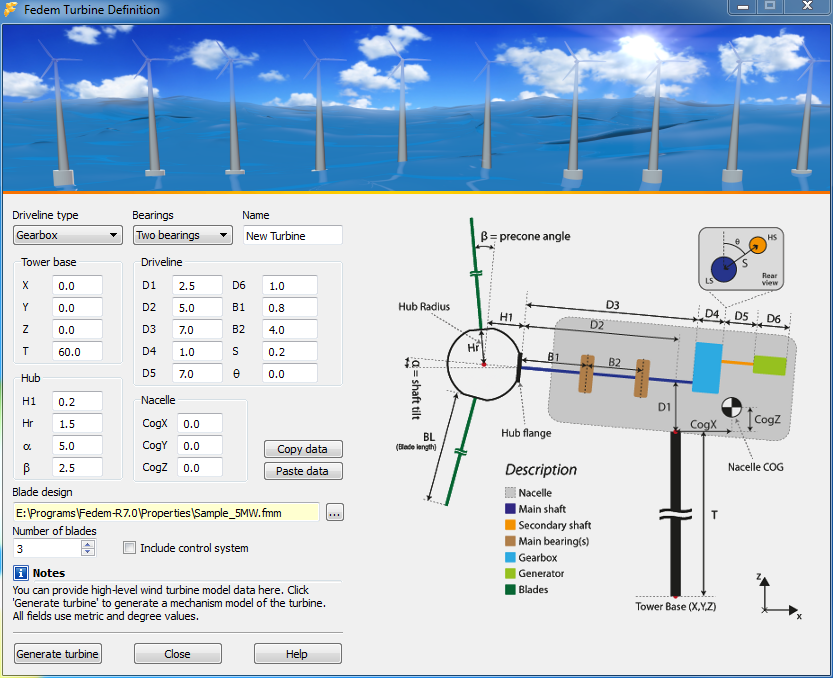
\includegraphics[width=\textwidth]{Figures/3b-TurbineDefinition}}
  \put(31,166){\Bullet{1}}
  \put(75,166){\Bullet{2}}
  \put(18,118){\Bullet{3}}
  \put(73,109){\Bullet{4}}
  \put(10,48){\Bullet{5}}
  \put(117,62){\Bullet{6}}
  \put(102,48){\Bullet{7}}
\end{picture}

The Turbine Definition dialog box is used to enable easy configuration and
creation of wind turbine models. All the fields have predefined default values,
so the only thing you need to do in order to generate a valid wind turbine model
is to click the \textbf{Generate turbine} button.

However, before that you may choose another {\sl Driveline type}, the number of
{\sl Bearings}, the {\sl Number of blades} as well as selecting a pre-defined
{\sl Blade design}. You may also specify a {\sl Name} for the turbine.
The figures on the next page illustrate the different driveline and bearing
configurations that are currently supported.

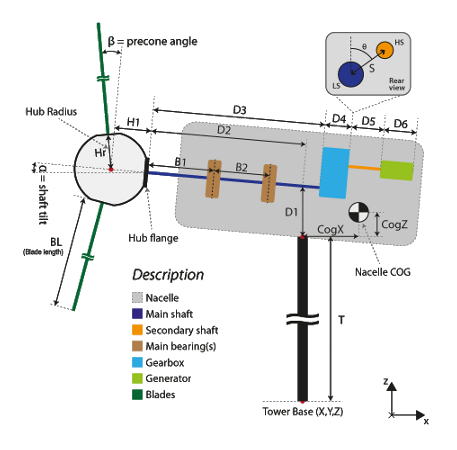
\includegraphics[width=0.43\textwidth]{Figures/3b-TurbineDefinition4}\hfill
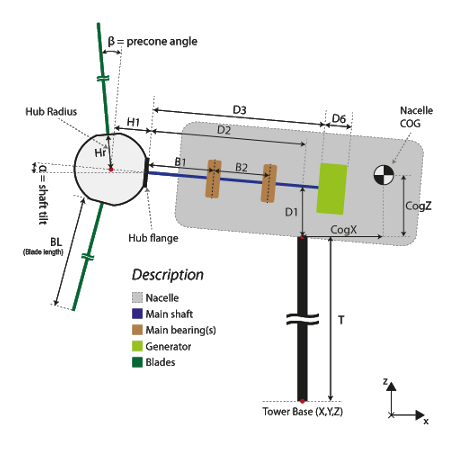
\includegraphics[width=0.43\textwidth]{Figures/3b-TurbineDefinition1}
\hspace*{0.1\textwidth} Gearbox, two bearings
\hspace*{0.3\textwidth} Direct, two bearings

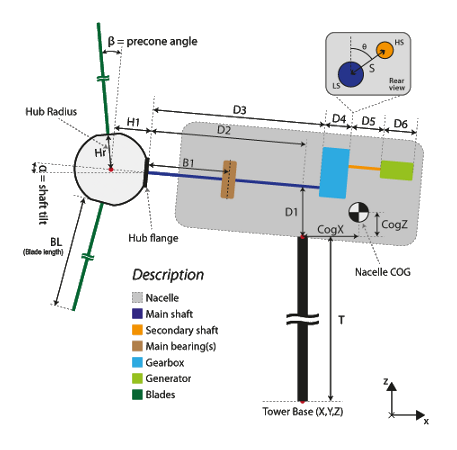
\includegraphics[width=0.43\textwidth]{Figures/3b-TurbineDefinition5}\hfill
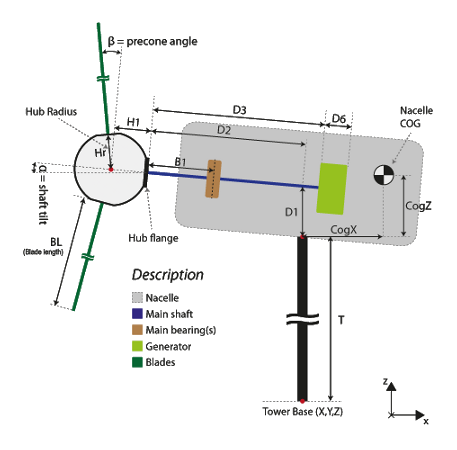
\includegraphics[width=0.43\textwidth]{Figures/3b-TurbineDefinition2}
\hspace*{0.1\textwidth} Gearbox, one bearing
\hspace*{0.3\textwidth} Direct, one bearing

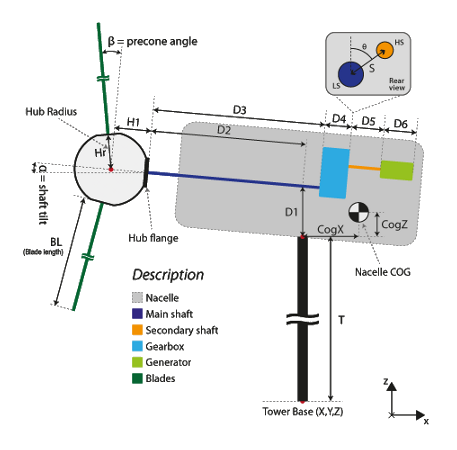
\includegraphics[width=0.43\textwidth]{Figures/3b-TurbineDefinition6}\hfill
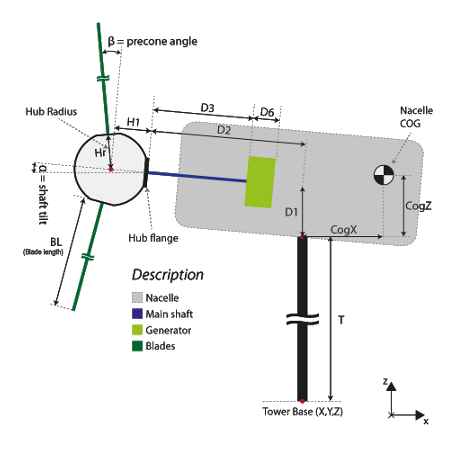
\includegraphics[width=0.43\textwidth]{Figures/3b-TurbineDefinition3}
\hspace*{0.1\textwidth} Gearbox, no bearings
\hspace*{0.3\textwidth} Direct, no bearings

The various fields in the Turbine Definition dialog box are as follows:

\begin{bulletlist}
\item{\sl Tower base} --
  These fields specify the turbine position and tower height:
  \vskip-\baselineskip
  \begin{itemize}
  \subitem{\sl X, Y, Z} --
    Global position of the bottom of the tower.
  \subitem{\sl T} --
    Height of the tower. Specify the value 0.0 to generate a turbine
    model without a separate Tower object.
  \end{itemize}

\item{\sl Driveline} --
  These fields specify the location and size of various items inside
  the turbine nacelle:
  \begin{itemize}
  \subitem{\sl D1} --
    Distance from the tower top to the main shaft.
  \subitem{\sl D2} --
    Distance from the tower top to the hub flange.
  \subitem{\sl D3} --
    Distance from gearbox to the hub flange. \newline
    This also equals the length of the main shaft.
  \subitem{\sl D4} --
    Depth of the gearbox.
  \subitem{\sl D5 } --
    Length of the secondary shaft.
  \subitem{\sl D6 } --
    Depth of the generator.
  \subitem{\sl B1} --
    Distance from the hub flange to the first bearing.
  \subitem{\sl B2} --
    Distance between the two bearings.
  \subitem{\sl S} --
    Offset distance between the shaft axes.
  \subitem$\theta$ --
    Offset angle of the secondary shaft.
  \end{itemize}

\item{\sl Hub} --
  These fields specify the positions and angles of the hub:
  \begin{itemize}
  \subitem{\sl H1} --
    Distance from the hub flange to the hub apex.
  \subitem{\sl Hr} --
    Radius of the hub.
  \subitem$\alpha$ --
    Uptilt angle of the main shaft.
  \subitem$\beta$ --
    Precone angle of the blades.
  \end{itemize}

\item{\sl Nacelle} --
  These fields provide information about the nacelle:
  \begin{itemize}
  \subitem{\sl CogX, CogY, CogZ} --
    Position of the center of gravity for the nacelle,
    relative to the top of the tower.
  \end{itemize}

\item{\sl Number of blades} --
  Specifies the number of blades for the turbine. Legal values are 2, 3 and 4.

\item{\sl Blade design} --
  Specifies the blade design to use. A set of sample blades are included with
  the Fedem Windpower installation. They are stored as separate model files and
  can be selected using the browse button \textbf{[...]}
  to the right of the blade design field.
  You can also make your own blade designs by using the Blade Definition
  dialog box, as shown in \refSection{blade-definition}{Blade definition}.

\EnumNote{The color of the Blade design field will be pink as long no valid path
  to a blade design file has been specified. It will change to yellow once
  a valid file path is entered. A green field means that this blade design
  is now included in the current model.}

\item{\sl Include control system} --
  If this toggle is enabled, a pre-defined control system for controlling
  the pitching and torque of the turbine will be generated,
  see \refSection{control-system}{Control system}.
\end{bulletlist}

The \textbf{Generate turbine} button will generate a mechanism assembly of
the defined turbine, consisting of beam elements, triads, joints, etc.
However, if turbine a model already has been created, the same button is
labeled \textbf{Update turbine} and the positions and properties of the
existing turbine components are then updated according the field values.

\Note{If a turbine model already exists, some of the fields in the dialog box
  cannot be changed and are therefore disabled (gray). These are
  \textbf{Driveline type}, \textbf{Bearings} and \textbf{Number of blades}.
  You must delete the existing model before these can be changed.}

The Turbine Definition dialog box also provides a \textbf{Copy data} button
and a \textbf{Paste data} button to simplify the process of experimenting with
many different turbine designs. Simply click the \textbf{Copy data} button to
copy the fields of the dialog box to the clipboard.
You can paste the data back into the dialog box by clicking \textbf{Paste data},
or paste the data to other applications.
The paste operation will not affect the disabled fields.


\SubSection{A newly generated wind turbinemodel}{newly-generated-wind-turbine}

The figure below illustrates a newly generated wind turbine model.
Here we have used the default values in the Turbine Definition dialog box,
and selected one of the sample blade designs included with the Fedem Windpower
installation.

After generating it, we have selected the turbine in the {\sl Objects} list
(i.e., the tree-node labeled ``New Turbine'' in the Model Manager panel), to
display the properties for the generated turbine object in the Property Editor
panel. The ``New Turbine'' node has also been expanded (by first clicking on
the ``+'' sign to the left of the Turbine icon,

\includegraphics[scale=0.45]{Figures/Icons/turbineDef}) to reveal some of the
other underlying components (``Nacelle'', ``Gearbox'', etc.)
making up the total turbine model.

The Turbine object and many of its sub-components are specializations of macro
objects referred to as sub-assemblies.
Their role is to create a natural hierarchy of the various model components,
to ease navigation within complex models
(see \refSection{sub-assemblies}{Sub-assemblies} for details).

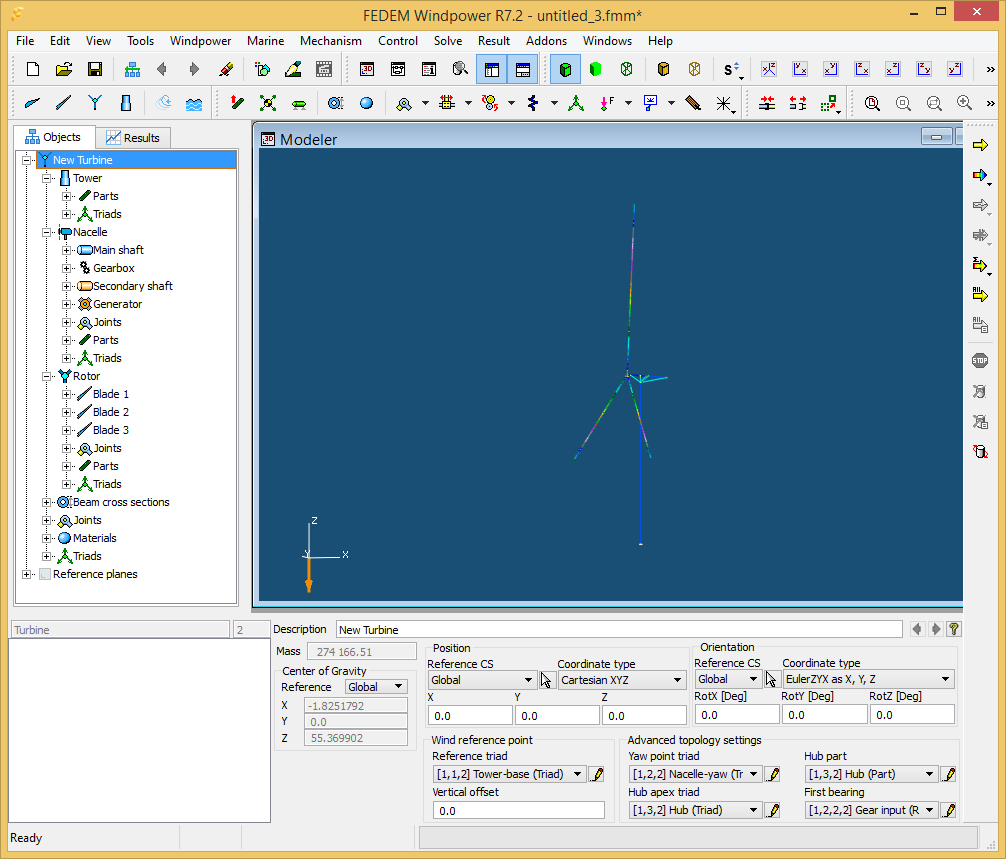
\includegraphics[width=0.96\textwidth]{Figures/3b-Main2}

In the {\sl Objects} list we see that the turbine model contains a tower,
a nacelle, a rotor, as well as joints and triads. Further down the tree,
we also see some beam cross sections, materials and so forth.
The model tree contains a large hierarchy of different mechanism elements.
When selecting any of these elements in the {\sl Objects} list,
we see the properties of the selected element in the Property Editor panel.
We will describe these elements and properties below.
For the basic elements, (parts, triads, joints, etc.),
refer to \refChapter{mechanism-elements}{Mechanism Elements}.

\SubSubSection{Turbine}{turbine}

The turbine object is, naturally, the main or top-level element in the model.
The Turbine includes Tower, Nacelle, Rotor, etc.
The Modeler view, in the center of the figure above, shows the various elements
of the model in 3D space. We use a scientific visualization to show the
3D position and orientation of each element in the model.
Even though you can click the various elements in the modeler, it is probably
easier and more logical to access the elements from the tree structure.

The figure below shows the properties of the turbine.
They are as follows:

\noindent
\begin{picture}(344,105)
  \put(0,0){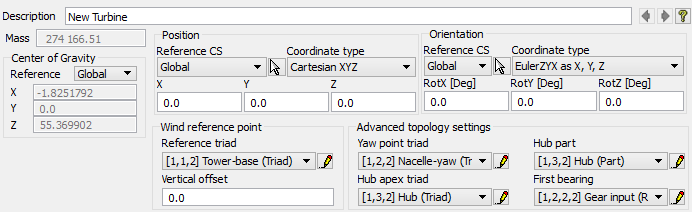
\includegraphics[width=\textwidth]{Figures/3b-TurbineProperty}}
  \put(100,83){\Bullet{1}}
  \put(243,83){\Bullet{1}}
  \put(50,81){\Bullet{2}}
  \put(50,46){\Bullet{3}}
  \put(130,37){\Bullet{4}}
  \put(245,37){\Bullet{5}}
\end{picture}

\begin{bulletlist}
\item{\sl Position and orientation} --
  These fields are used to modify the position and orientation of the entire
  turbine assembly. The {\sl X}, {\sl Y} and {\sl Z} fields specify the position
  whereas the {\sl RotX}, {\sl RotY} and {\sl RotZ} fields rotate the turbine.
  Advanced users may wish to explore the {\sl Reference CS}
  (reference coordinate system) and {\sl Coordinate type} fields.
  See \refSection{origin-property}{Origin property}
  for a further description of these fields.
\item{\sl Mass} --
  This field reports the total mass of the whole turbine assembly.
  The mass is provided in kilograms when the model is built in SI units.
  The total mass is updated automatically, whenever the mass property or
  size of any of the sub-components of the turbine is changed.
\item{\sl Center of Gravity} --
  These fields report the location of the turbine's center of gravity,
  in either Global coordinates or in Local coordinates with respect to
  the origin of the turbine assembly. The center of gravity is updated
  automatically, whenever the mass property or size of any of the
  sub-components of the turbine is changed.
\item{\sl Wind reference point} --
  These fields specify a Triad and a vertical offset that together
  define the reference point (origin) for the wind field.
\item{\sl Advanced topology settings} --
  These settings are used to correct/reassign certain triads, parts and joints
  that can become lost when modifying the components of the turbine.
  If you for example were to delete the tower of the turbine,
  you would see that the Reference triad and the Yaw point triad will be
  unassigned. If you later add a tower manually,
  you would have to assign these fields proper values.
\end{bulletlist}

\SubSubSection{Tower}{tower}

The tower of the wind turbine is represented with the Tower object in
the {\sl Objects} list. The default representation consists of a Generic Part
and a Triad in each end. A tower model may have to be more complex than that,
and other ways modeling the tower are given in
\refSection{tower-definition}{Tower definition}.

\Note{A valid wind turbine model is not required to contain a separate Tower
object. The tower may optionally be an integrated part of the underlying
support structure. It may then be modeled manually, by importing a FE
part or through other means. In these cases, the turbine model needs to
be generated with the tower height set to zero (see bullet \TextBullet{1} in
\refSection{turbine-definition}{Turbine definition}).}

\begin{wrapfigure}[7]{r}{0.25\textwidth}
  \vskip-\baselineskip
  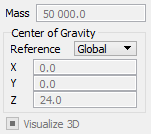
\includegraphics[width=0.25\textwidth]{Figures/3b-TowerProperty}
\end{wrapfigure}

When the tower object is selected in the {\sl Objects} list, the total mass
(in kilograms) of the tower and its center of gravity position are displayed
in the property panel, as shown at right.
The {\sl Visualize 3D} toggle (active only if the tower consists of beam
elements), can be used to quickly toggle on/off the 3D visualization of
all the beam elements the tower consists of, see also bullet \TextBullet{3}
in \refSection{beam-properties}{Beam properties}.

\Note{The Visualize 3D toggle in the Tower property panel
  has a tri-state value. In addition to the usual
  on 
\includegraphics[scale=0.5]{Figures/Icons/on}
  and off 
\includegraphics[scale=0.5]{Figures/Icons/off} states,
  it can also have a neither-on-nor-off
  
\includegraphics[scale=0.5]{Figures/Icons/onoff} state, in which
  the corresponding on or off settings on each element are applied instead.
  This is usually the default setting for such tri-state toggles.}

\SubSubSection{Nacelle}{nacelle}

The nacelle object contains the generator and associated parts,
such as the main shaft, secondary shaft, gearbox, etc. Many of the elements
in the nacelle will affect the behavior of the wind turbine.
Unless there are some limits on the behavior of the turbine, it will for example
rotate freely when you apply a wind field. A real turbine offers resistance to
a wind field, and has limits on rotational velocity, etc.
The main nacelle components are described below.

There are also additional elements in the nacelle object,
such as the nacelle {\sl Part} representing the nacelle structure itself,
the revolute joints for the bearings, and various triads.
See \refChapter{mechanism-elements}{Mechanism Elements}
for a full description of those object types.
Fedem Windpower also supports adding a full control system,
as will be discussed in \refSection{control-system}{Control system}.

\SubSubSection{Driveline and Generator}{driveline-and-Generator}

The generator basically contains a revolute joint and its master triad
connecting the generator to the nacelle part. The properties of the
generator object are illustrated in the figure below.

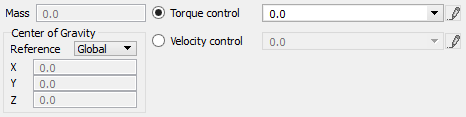
\includegraphics[width=0.72\textwidth]{Figures/3b-Generator}

The generator properties consists of the Mass and Center of Gravity fields,
which have similar meaning as for the other turbine sub-components. In addition,
it has settings for controlling the torque or velocity of the generator.

The Torque control toggle can be used to assign a load to the generator,
whereas the Velocity control toggle can be used to set a prescribed velocity.
You can enter a specific value in either of these two fields.
You can also choose a function here which can be created by choosing
\textbf{Function} on the {\sl Mechanism} menu or the Right-click menu in the
{\sl Objects} list (see \refSection{creating-a-function}{Creating a function}).
All existing functions will then be available in the Torque and Velocity control
drop-down lists.

If you expand the tree-list of the generator and select the Generator
revolute joint, you will see that the Rz-values of this joint are
updated when you change the properties of the generator. You can model
more advanced representations or use a control system, as discussed later,
if you wish to do more advanced modeling. In this basic introduction,
you can leave the properties as they are by default, but add a load
or set the prescribed velocity. This will make the turbine model behave more
like a real turbine, since the generator is the main load of a wind turbine.

Depending on the Driveline type selected, the driveline contains:

\begin{itemize}
\item{\sl Gearbox} --
  A driveline with a gear box contains a main shaft and
  a secondary (high-speed) shaft.
\item{\sl Direct} --
  A direct driveline contains a main shaft only.
\end{itemize}

The driveline may optionally have zero, one or two bearings, depending on what
you selected when you created the turbine. The main shaft will contain one,
two or three beam elements depending on the number of bearings added.

The gear box driveline also has a gearbox object that contains:

\begin{itemize}
\item{\sl A gear} --
  The gear basically specifies the transmission output ratio.
  You will find the gear inside the Gearbox in the tree-list.
  When you select the gear, the properties will display the transmission
  output ratio.
\item{\sl Two revolute joints} --
  The gearbox includes two revolute joints, one at each end of the gear.
\item{\sl Two triads} --
  The gear box also includes two master triads for each joint,
  connecting the gear box to the nacelle part.
\end{itemize}

\SubSubSection{Shaft}{shaft}

The figure below illustrates the properties for the main and secondary shafts.
It is essentially identical to the property panel of the Beam elements,
described in \refSection{beam-properties}{Beam properties},
except for the {\sl Notes} in the bottom of the frame, and that the
{\sl Visualize 3D} toggle here has a similar tri-state behavior as
explained above for the \protect\hyperlink{tower}{\sl Tower}.

\noindent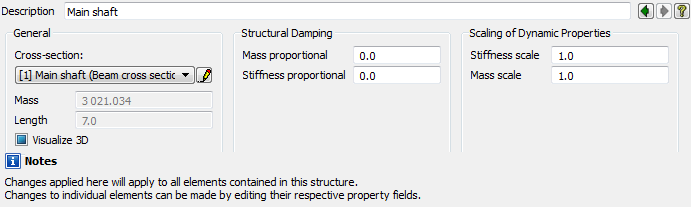
\includegraphics[width=\textwidth]{Figures/3b-MainShaft-Prop}

The {\sl Mass} and {\sl Length} fields of the Shaft property panel display the
sum of the corresponding mass- and length fields of all the beam elements
that the shaft consists of.

Editing any of the {\sl Structural Damping} or
{\sl Scaling of Dynamic Properties} fields, the values entered will apply to
all the underlying beam elements of the shaft, which can be verified
by selecting any of the beam elements. However,
if such a field is edited for at least one beam element such that the beams
making up a shaft no longer have identical properties,
the corresponding field in the {\sl Shaft} property panel will be blank
(i.e., no value is displayed).

\SubSubSection{Rotor}{rotor}

The rotor basically consists of the blades and the hub. Fedem Windpower
enables you to design your own blades, using any number of Airfoil data
sets for the blades, to set the air environment, etc., as we will see in
\refSection{creating-an-advanced-wind-turbine-model}
           {Creating an advanced wind turbine model}.
But, in this basic introduction, we just use a typical three-blade
configuration using the sample blade design ``Sample\_5MW''
that comes with the installation.

In the {\sl Objects} list, we see that the rotor contains the following:

\begin{itemize}
\item{\sl Three blades} --
  These objects represent the turbine blades.
  Beneath each blade you will find a list of beams and triads that the
  blade consists of. The blade modeling iself is discussed in
  \refSection{blade-definition}{Blade definition}.
\item{\sl Three revolute joints} --
  These are the pitch joints of the blades.
  The pitch controller basically adjusts the angular motion in these joints.
\item{\sl A rigid joint} --
  This is the joint that connects the main shaft to the hub part in the rotor.
\item{\sl The hub part} --
  This is a Generic part representing the hub itself.
  Each arm of the hub is connected to a pitch joint.
\item{\sl Four triads} --
  These are triads used to connect the parts and joints.
\end{itemize}

The figure below illustrates the properties for a blade object.

\noindent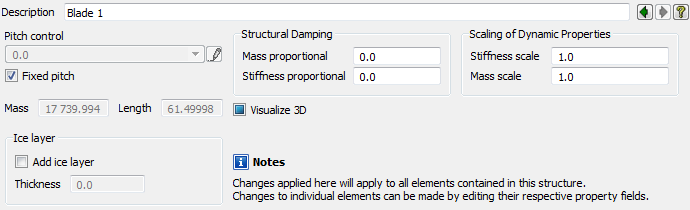
\includegraphics[width=\textwidth]{Figures/3b-Blade-Prop}

The {\sl Pitch control} is used to control the pitching angle.
It can either be fixed or prescribed. In the latter case, either a constant
value or a function can be assigned to describe the actual pitch angle.
The setting of the {\sl Pitch control} field is also reflected in the Rz-values
of the corresponding revolute joint, which can be edited if more advanced pitch
modeling is needed, e.g., adding flexibility and damping in the pitching motors,
etc.

The blade property panel also include fields for total mass and length,
which are useful for verifying the model before simulation.
It also has a {\sl Visualize 3D} toggle with similar operation as for the
\protect\hyperlink{tower}{\sl Tower} and \protect\hyperlink{shaft}{\sl Shaft}
objects described above, as well as {\sl Structural Damping} and
{\sl Scaling of Dynamic Properties} fields with similar functionality
as for the \protect\hyperlink{shaft}{\sl Shaft}.

You can also add a ice layer, resulting in extra non-structural mass on
the blade. The ice mass is estimated based on a mass density of 0.917 kg/m$^3$
and an ellipsoidal cross section, using the specified {\sl Chord length}
and {\sl Thickness ratio} parameters of the
\protect\hyperlink{blade-definition}{\sl Blade definition} to deduce the
length of the principal axes of the ellipse.

\clearpage


%%%%%%%%%%%%%%%%%%%%%%%%%%%%%%%%%%%%%%%%%%%%%%%%%%%%%%%%%%%%%%%%%%%%%%%%%%%%%%%%
\Section{Basic solving and analysis}{basic-solving-and-analysis}

After creating a basic wind turbine model, we can ``solve'' that model.

If you are new to this, you are probably wondering what ``solving'' is.
Well, solving is basically the process of (1) mathematically reducing
the turbine model into a smaller and easier-to-manage internal model that can
be solved numerically, and then to (2) make an animated physics model
of the wind turbine.

After running the Fedem dynamics solver, you will be able to play an animation
where you can see the effect of all loads and environmental conditions acting
on the turbine. If you, for example, have used a too thin tower,
you may see it break down when the wind speeds get too high.

Fedem Windpower also contains tools like Simulation events that enables
you to set up and test a range of changing conditions,
to see how the wind turbine behaves in response to these events.

We will only describe basic solving in this section,
whereas \refSection{dynamics-analysis}{Dynamics analysis}
contains full details about the solving process. It is recommended to
read that part before using the results in an actual project.
Good and usable results are highly dependent on the analysts experience,
and correct application of modeling, solving and analysis.

\clearpage

\SubSection{Running the dynamics solver (basic mode)}
           {running-the-dynamics-solver-basic-mode}

\IconTextFirst{solve}{
  You can display the Dynamics Solver Setup dialog box (shown below) by
  choosing \textbf{Dynamics Solver (Basic Mode)...} on the
  {\sl Solve} menu, or by clicking the associated button on the
  {\sl Solvers} tool bar.}

\includegraphics[width=0.58\textwidth]{\ReferenceImg/dlg-solver-basic1}

In this dialog box you can adjust the {\sl Start} and {\sl Stop time}
of the simulation, as well as the {\sl Time increment} size to use.
Please refer to
\refSection{dynamics-solver-basic-mode}{Dynamics Solver (Basic Mode)}
for details on all fields of the dialog box.

Wind turbine simulations usually need to be performed over a relatively long
time span and the default stop time is typically 1.0. Therefore, at least
you will need to edit this field before starting the solver.

When finished defining the simulation setup, click the \textbf{Run!} button
to start the dynamics solver. The solver will then run in the background as
a separate process, such that you can continue browsing the model, etc.,
while it is running. It is not possible to modify anything though,
when solver has started producing results data on secondary storage.


\SubSection{Basic results overview}{basic-results-overview}

If everything went well,
and no error messages have been reported in the output list,
then we will now have a result database that can be looked at in more detail.
If we click the {\sl Results} tab on top of the Model Manager panel on the left
side of the main window, we will see a set of predefined curves under the
{\sl Graphs} node, as shown below.

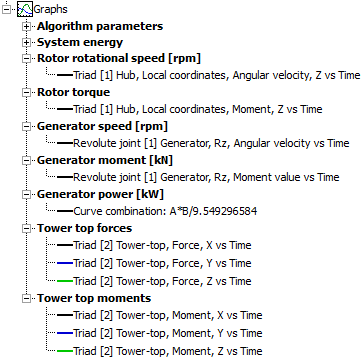
\includegraphics[width=0.68\textwidth]{Figures/3b-Graphs1}

These curves are as follows:

\begin{itemize}
\item{\sl Algorithm parameters} --
  Contains curves monitoring the solution algorithm performance
  (not important for our basic results review).
\item{\sl System energy} --
  Contains curves plotting various system energy quantities,
  to verify global energy conservation (not important now).
\item{\sl Rotor rotational speed [rpm]} --
  The angular velocity of the turbine rotor.
\item{\sl Rotor torque} --
  The torque of the rotor.
\item{\sl Generator speed [rpm]} --
  The rotational speed of the rotor.
\item{\sl Generator moment [kN]} --
  The generator moment.
\item{\sl Generator power [kW]} --
  The generator power generation.
\item{\sl Tower top forces} --
  Force components on the top of the tower.
\item{\sl Tower top moments} --
  Moment components on the top of the tower.
\end{itemize}

You can right click a graph (bold text) or a curve under a graph to choose
{\sl Show Graph}. If no graph is displayed, it might be due to a solver error.
In that case, refer to \refSection{dynamics-analysis}{Dynamics analysis}
for trouble-shooting.

The figures below illustrate the graphs that will be displayed when you
choose to show them after running the dynamics solver. To learn more on
graphs and curves in Fedem, see \refSection{graphs}{Graphs}.

\noindent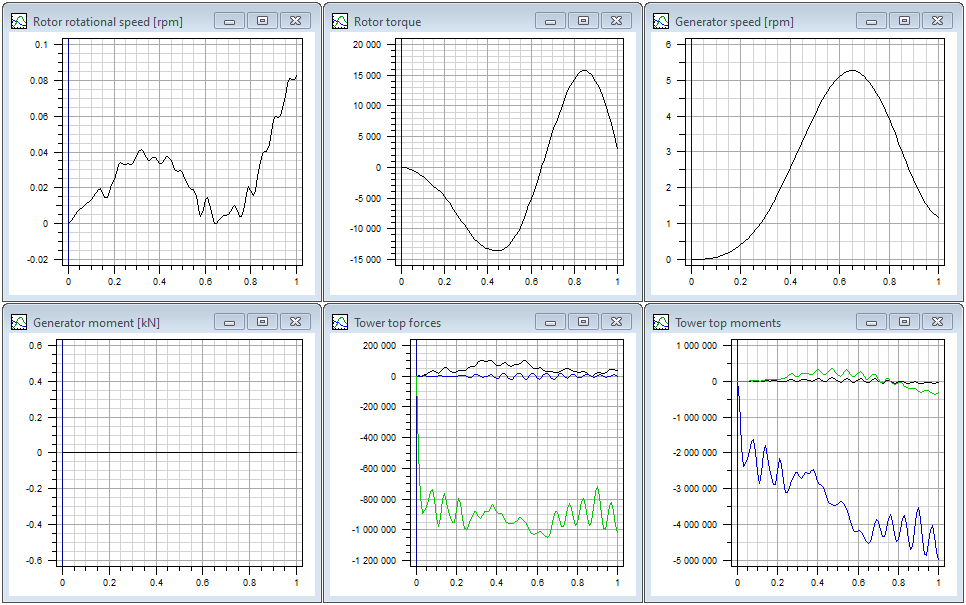
\includegraphics[width=\textwidth]{Figures/3b-Graphs2}


\SubSection{Reliability and validity of results}
           {reliability-and-validity-of-results}

The reliability and validity of the results is a very important topic.
It is the highest priority for Fedem to ensure reliable and valid results.
{\sl Reliability} is the consistency of a result, or the degree to which
a result provides the same results every time it is used under the same
conditions. {\sl Validity} is focused on whether a result is valid.

Fedem Windpower uses AeroDyn for calculation of the forces due to wind on the
blade elements. AeroDyn bases its calculations on provided input on the air
environment, updated positions and velocities of the wind turbine, and airfoil
tables with drag and lift coefficients. The output forces on the blade elements
are used by our solvers to provide results that can be analysed.
The reliability and validity evaluations/certifications of the AeroDyn
implementation are available at the National Renewable Energy Laboratory
(see \href{https://wind.nrel.gov/}{wind.nrel.gov}).


%%%%%%%%%%%%%%%%%%%%%%%%%%%%%%%%%%%%%%%%%%%%%%%%%%%%%%%%%%%%%%%%%%%%%%%%%%%%%%%%
\Section{Creating an advanced wind turbine model}
        {creating-an-advanced-wind-turbine-model}

One of Fedem Windpower's greatest strengths is the ability to do very advanced
and highly customized modeling tasks, while at the same time being easy and
effective to use. We will in this section look in more detail at some advanced
wind turbine modeling issues which may be used to customize the wind turbine
model before the numerical simulation is performed. These are as follows:

\begin{itemize}
\item\protect\hyperlink{airfoil-definition}{\sl Airfoil definition} --
  The Airfoil Definitions dialog box specifies the aerodynamic cross section
  properties of the wind turbine blades. The airfoil data is stored on
  external files and used by the {\sl Blade Definitions} to describe
  the design of the turbine blade to be used. Since these files are read
  directly by AeroDyn their format is accordingly.
\item\protect\hyperlink{blade-definition}{\sl Blade definition} --
  The Blade Definition dialog box specifies a wind turbine blade design.
  Both aerodynamic and structural properties are specified here.
  The aerodynamic properties are used by AeroDyn to calculate forces on the
  turbine blades which are applied as loads on the structural model.
\item\protect\hyperlink{aerodynamic-setup}{\sl Aerodynamic setup} --
  The Aerodynamic Setup dialog box is used to specify the global air
  environment for the wind turbine, that is, the specification of the
  wind field to use, deterministic or turbulent. It also contains some
  fields with control parameters for AeroDyn.
\item\protect\hyperlink{sea-environment}{\sl Sea environment} --
  The Sea Environment dialog box is used to specify the sea environment for
  an offshore wind turbine. We can here specify the mean sea level, water depth,
  water density, functions for waves and current, etc.
  Refer to \refSection{sea-environment}{Sea environment}
  for a detailed description of this dialog box.
\item\protect\hyperlink{tower-definition}{\sl Tower definition} --
  The Tower Definition dialog box is used to define a more advanced tower model
  than the default tower representation generated via the
  \protect\hyperlink{turbine-definition}{\sl Turbine definition} dialog box.
  The Tower Definition dialog box offers an intermediate complex turbine tower.
  Even more advanced towers can be modeled by importing FE-models.
\item\protect\hyperlink{control-system}{\sl Control system} --
  The Control system is used to make functions that can monitor and modify
  properties in the wind turbine model. The wind turbine that is created by the
  \protect\hyperlink{turbine-definition}{\sl Turbine definition} dialog box
  can use an optional default control system, that makes the turbine
  behave more like a real wind turbine with limited rotational speed,
  pitch controller, torque controller, etc.
\end{itemize}


\SubSection{Airfoil definition}{airfoil-definition}

The purpose of the Airfoil Definitions dialog box is to facilitate the creation
of a set of airfoils to use in the turbine blade definition.
An airfoil is basically a cross section of the blade where different aerodynamic
properties (drag and lift coefficients, etc.) are specified around the blade.

Fedem Windpower uses the AeroDyn airfoil format of NREL.
The Airfoiil Definition dialog box is simply an editor for such files.
For information on this format, see
\href{https://www.nrel.gov/wind/nwtc/aerodyn.html}
     {nrel.gov/wind/nwtc/aerodyn.html}.

The airfoil files are referred to when designing the blades, in the
\protect\hyperlink{blade-definition}{\sl Blade definition} dialog box,
and when the completed turbine model is being solved, the used airfoil files
will be read by AeroDyn (via the dynamics solver) to calculate the wind loads.

The Airfoil Definition dialog box is shown below:

\noindent
\begin{picture}(344,305)
  \put(0,0){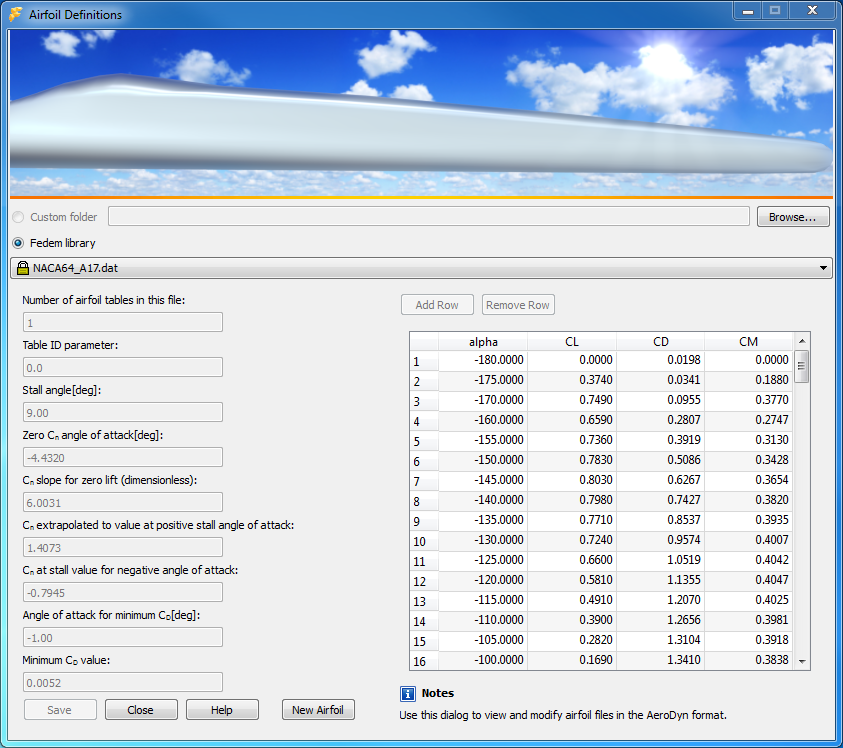
\includegraphics[width=\textwidth]{Figures/3b-AirfoilDefinition}}
  \put(-9,206){\Bullet{1}}
  \put(50,190){\Bullet{2}}
  \put(90,169){\Bullet{3}}
  \put(90,151){\Bullet{4}}
  \put(90,132){\Bullet{5}}
  \put(92,59){\line(1,0){5}}
  \put(97,59){\line(0,1){68}}
  \put(92,127){\line(1,0){5}}
  \put(95,95){\Bullet{6}}
  \put(92,21){\line(1,0){5}}
  \put(97,21){\line(0,1){35}}
  \put(92,56){\line(1,0){5}}
  \put(95,35){\Bullet{7}}
  \put(240,172){\Bullet{8}}
\end{picture}

\begin{bulletlist}
\item
  These two radio buttons allow you to select whether to use the
  airfoils provided with the installation ({\sl Fedem library}),
  or from a {\sl Custom folder,} that may be selected using the
  \textbf{Browse...} button.
\item
  This drop-down menu allows you to select the name of the airfoil file
  to be used. If using airfoils from the {\sl Fedem library}, their
  properties can not be edited, which is indicated by the lock symbol.
\item{\sl Number of airfoil tables in this file} --
  The airfoil file format is designed so that they can contain
  several actual airfoil tables.
  The airfoil file in the figure above contains a single table only.
\item{\sl Table ID parameter} --
  Identifier for each airfoil table.
\item{\sl Stall angle [deg]} --
  The stall angle, in degrees, of this airfoil.
\item
  The next four parameters characterize the normal force coefficient ({\sl Cn}).
  Refer to the User's Guide and the AeroDyn Theory Manual of AeroDyn
  for the interpretation of these parameter values.
\item
  The next two parameters specify the minimum drag coefficient ({\sl CD}).
  These two values can be deduced from the tabulated {\sl CD}-values
  on the right side of the dialog box.
\item
  On the right side of the dialog box, we find the airfoil table data
  with the following columns:
  \begin{itemize}
  \subitem{\sl alpha} -- The angle of attack.
    The table must be written in order of increasing angle of attack.
    It is preferable to use a table for angles between -180 to +180 degrees.
    The coefficient values should be the same at -180 and +180 degrees
    to avoid discontinuity.
  \subitem{\sl CL} -- Static lift coefficient for this angle of attack.
  \subitem{\sl CD} -- Drag coefficient for this angle of attack.
  \subitem{\sl CM} -- Pitching moment coefficient for this angle of attack.
  \end{itemize}
  The \textbf{Add Row} button adds an empty row (all values zero) at the bottom
  of the table. The \textbf{Remove Row} button deletes the last row.
\end{bulletlist}

The \textbf{New Airfoil} button creates a new, empty,
airfoil and is placed in the current {\sl Custom folder}
(you can't create new airfoils in the {\sl Fedem library}).
The \textbf{Save} button writes the current dialog box content to the
airfoil file.
For more information, please see the AeroDyn User's Guide, available from
\href{https://www.nrel.gov/wind/nwtc/aerodyn.html}
     {nrel.gov/wind/nwtc/aerodyn.html}.

We have included a set of sample airfoil files, provided by NREL, with the
Fedem Windpower installation. In some projects, the actual blade design is of
less concern, and then using these airfoils will be satisfactory.
But, in other projects, the user may wish to provide their own airfoils.


\SubSection{Blade definition}{blade-definition}

Fedem Windpower includes some sample blade designs
(e.g., the file ``Sample-5MW'') within the installation.
You can just specify one of these sample blades in the
\protect\hyperlink{turbine-definition}{\sl Turbine definition} dialog box,
if the blades of the turbine are not the main focus area for your simulation.
However, most projects will require that the blades are defined in detail for
that project. This is performed in the Blade Definition dialog box, shown below.

\noindent
\begin{picture}(344,307)
  \put(0,0){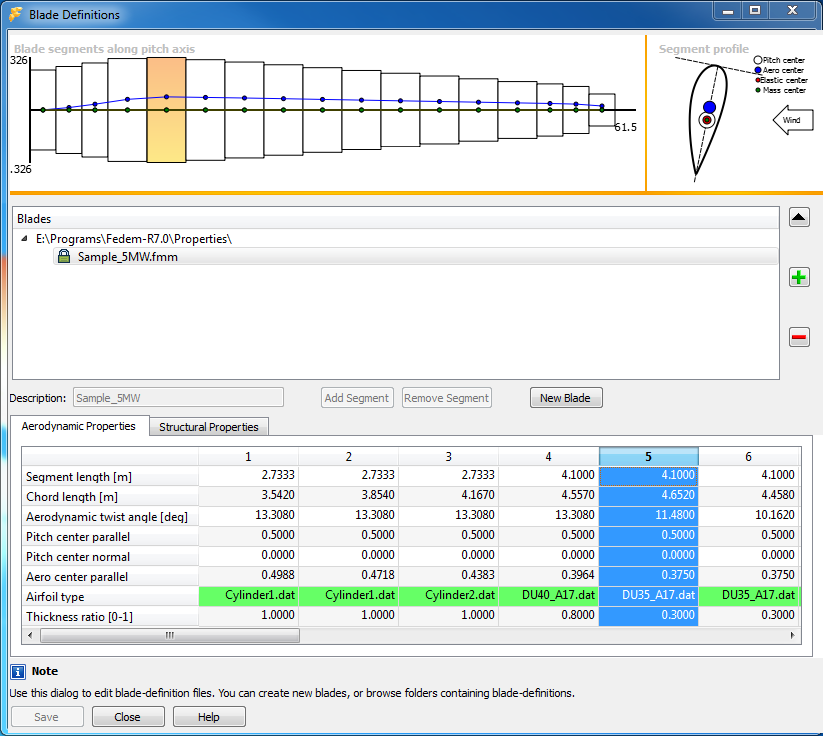
\includegraphics[width=\textwidth]{Figures/3b-BladeDefinition1}}
  \put(200,280){\Bullet{1}}
  \put(100,210){\Bullet{2}}
  \put(118,137){\Bullet{3}}
  \put(55,115){\Bullet{4}}
\end{picture}

The Blade Definition dialog box consists of four main parts:

\begin{bulletlist}
\item{\sl Blade visualization area} --
  The blade segment length and Chord length are visualized in the top left side
  of the dialog box, and the blade cross section for the selected segment
  is visualized in top right side.

\item{\sl Blades area} --
  Beneath the blade visualization, a list of file paths to the available blade
  designs are shown. Just click on a file name to display its properties in the
  visualization area and in the data table below.

  Use the green \textbf{+} button and the red \textbf{-} button to the far right
  to browse for new libraries of blade designs, or to remove a selected folder
  from the {\sl Blades} list. Blades that are included with the installation are
  not editable, as indicated by the lock symbol.

\item{\sl Description} --
  In the description field you can assign a name to the blade.
  Next to it you find the \textbf{Add Segment} and \textbf{Remove Segment}
  buttons, which are used to add a new column in the data table,
  and to remove the currently selected column (or the last one if none were
  selected), respectively.
  The \textbf{New Blade} button can be used to create a completely new,
  initially empty, blade design.

\item{\sl Data table} --
  The table in the lower part of the dialog box contains the {\sl Aerodynamic}
  and {\sl Structural Properties} in separate tabs (see below).
  The blades are discretized into a limited number of segments with constant
  cross section properties, and each column of the table represents one
  blade segment. If you click on a column, its properties are illustrated
  in the upper right part of the dialog box.
\end{bulletlist}

The figure above shows the Blade Definition dialog box when it displays the
{\sl Aerodynamic Properties} of the blade segments.
It contains the following rows:

\begin{itemize}
\item{\sl Segment length [m]} --
  The length of each blade segment, along the pitch axis of the blade.
\item{\sl Chord length [m]} --
  Width of the blade segment (perpendicular to the length of the blade),
  edge to edge.
\item{\sl Aerodynamic twist angle [deg]} --
  Twist (in degrees) of the blade for this segment
  (labeled $\alpha$ in the figure below), relative to the rotor plane.
\item{\sl Pitch center parallel} --
  Location of the pitch center along the chord line ({\sl a}),
  given as a fraction of the chord length.
  This value is typically in the range [0,1], but can be negative if the center
  is located in front of the leading edge, and larger than one if it is located
  behind the trailing edge.
\item{\sl Pitch center normal} --
  Pitch center offset from the chord line in the normal direction ({\sl b}),
  given as a fraction of the chord length.
\item{\sl Aero center parallel} --
  Location of the aero center along the chord line ({\sl c})
  relative to the leading edge, given as a fraction of the chord length.
\item{\sl Airfoil type} --
  File name of the airfoil data for this blade segment.
  If you click on the file name a browse button \textbf{[...]} appears
  besides it, and by clicking that one you can browse for another airfoil file.
  See \refSection{airfoil-definition}{Airfoil definition}
  above for more details on the airfoils.
\clearpage
\item{\sl Thickness ratio [0-1]} --
  Thickness of the blade relative to the chord length.
  This value is only used to estimate the circumference of the cross section
  when calculating the weight of ice on the turbine blades
  (see \refSubSection{rotor}{Rotor}{newly-generated-wind-turbine}.
  It does not affect the aerodynamic load calculations.
  In addition, this value is also used to create the cross section visualization
  in the upper right part of the dialog box.
\end{itemize}

\phantomsection\label{blade-profile}{}
\noindent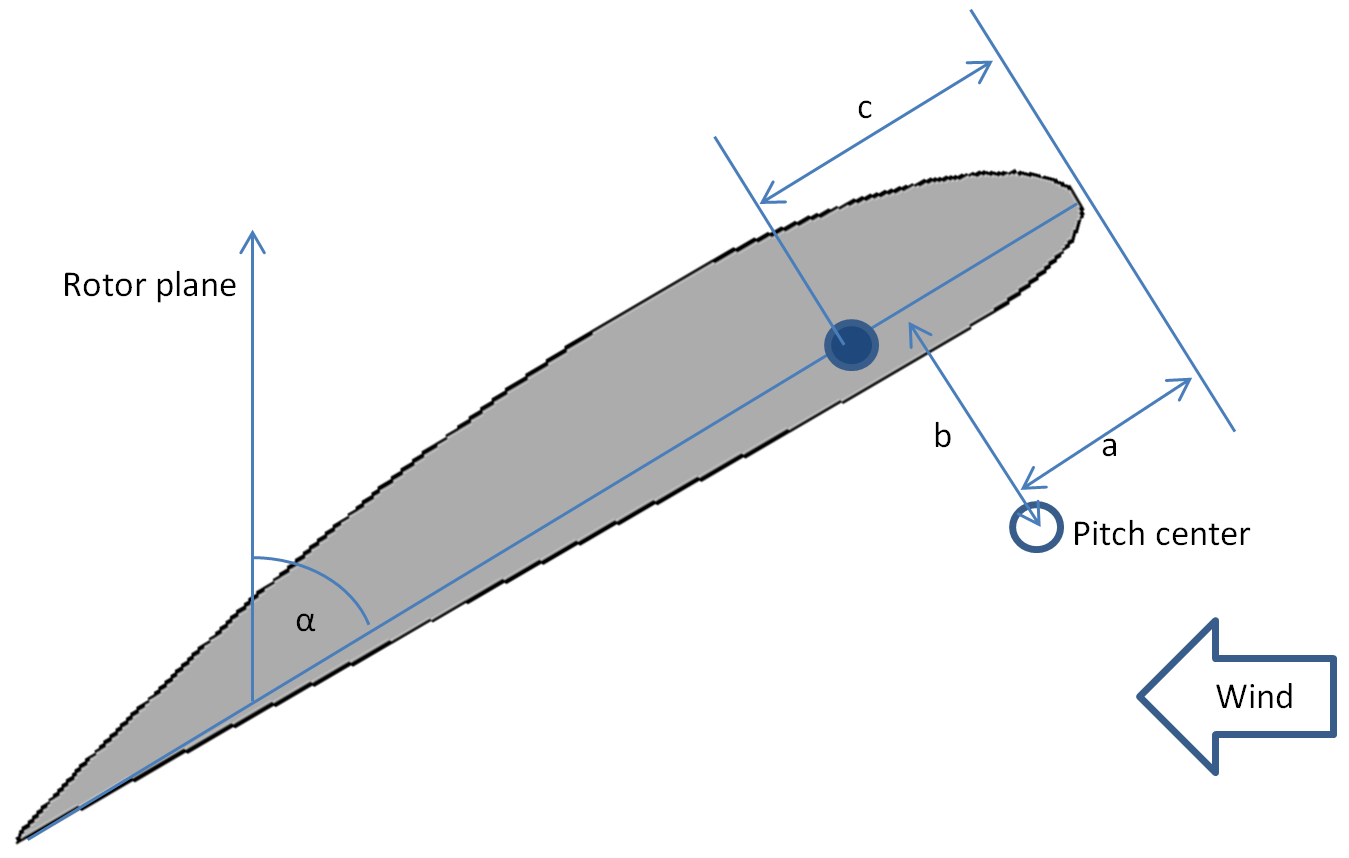
\includegraphics[width=\textwidth]{Figures/3b-BladeDefinition1-fig1}

The figure below shows the Blade Definition dialog box when it displays
the {\sl Structural Properties} of the blade segments. In this figure,
the {\sl Blades} area has also been contracted to show only the path of
the currently selected blade design. It can be expanded again (as in the
figure on \hyperref[blade-definition]{page \thechapter-21} by clicking the black
triangle to the right of the file path.

Above the {\sl Structural Properties} table, there are four toggles
that can enable or disable the different stiffness terms. When disabled,
the associated rows are hidden from the table.

\Note{The purpose of the stiffness toggles is to provide a simple means to
create a structural model of the blade when not all stiffness properties
are known. By disabling either the Bending, Axial or Torsional stiffness
fields, their actual values are replaced by some internally computed
large values, large enough to ensure that the associated deformations
become negligible. For the shear stiffness toggle, this is not needed,
as the beam formulation used allows for neglection of shear deformation
simply by setting the shear stiffnesses to zero.}

\noindent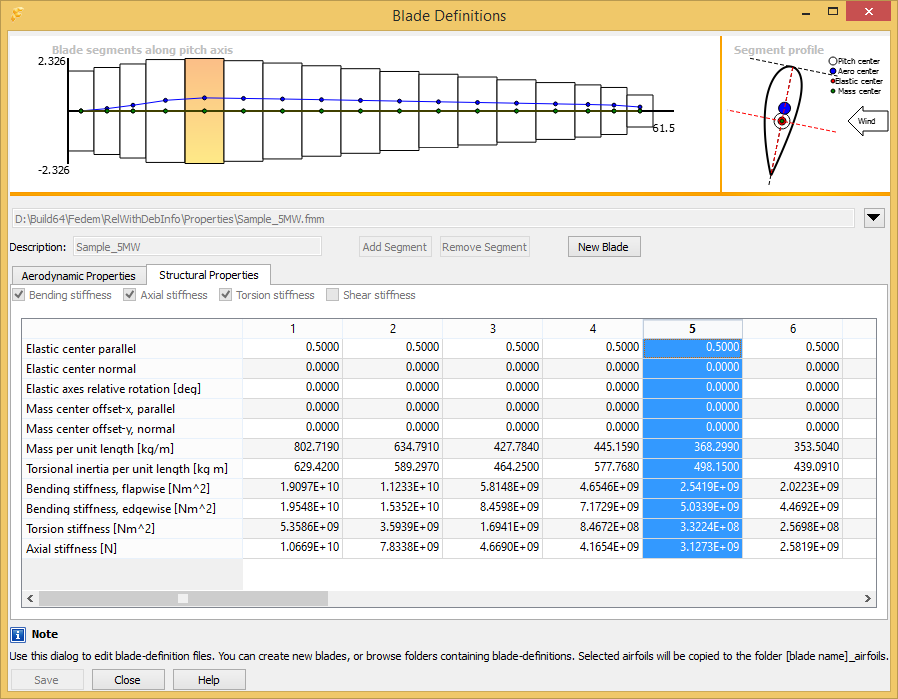
\includegraphics[width=\textwidth]{Figures/3b-BladeDefinition2}

When all the stiffness toggles are enabled, the {\sl Structural Properties}
table consists of the following rows:

\begin{itemize}
\item{\sl Elastic center parallel} --
  Location of the elastic center (also known as the neutral axis)
  along the chord line, given as a fraction of the chord length.
  This value is typically in the range [0,1], but can be negative if the center
  is located in front of the leading edge, and larger than one if it is located
  behind the trailing edge.
\item{\sl Elastic center normal} --
  Elastic center offset from the chord line in the normal direction,
  given as a fraction of the chord length.
\item{\sl Elastic axes relative rotation [deg]} --
  Angle (in degrees) between the chord line and the local y-axis of the
  structural beam element, for which the flap-wise bending stiffness is
  referring to. The edge-wise bending stiffness is then referring to the
  local z-axis, defined via the cross product of the length axis of the
  beam and the local y-axis.
\item{\sl Mass center offset, parallel and normal} --
  These two values specify the offset of the mass center from the
  elastic center, along the rotated elastic axes,
  given as fractions of the chord length.
\item{\sl Mass per unit length [kg/m]} --
  Mass density of this blade segment.
\item{\sl Torsional inertia per unit length [kg m]} --
  Torsional inertia of this blade segment.
\item{\sl Bending stiffness, flap-wise and edge-wise [Nm$^2$]} --
  These two values specify the bending stiffnesses $EI_{yy}$ and $EI_{zz}$,
  respectively, with respect to the local elastic axes defined by the
  {\sl Elastic axes relative rotation}.
\item{\sl Torsion stiffness [Nm$^2$]} --
  The torsional stiffness ($GI_t$).
\item{\sl Axial stiffness [N]} --
  The axial stiffness ($EA$).
\item{\sl Shear stiffness, flap-wise and edge-wise [N]} --
  These two values specify the shear stiffnesses $GA_{sy}$ and $GA_{sz}$,
  respectively, with respect to the local elastic axes.
\item{\sl Shear center, parallel and normal} --
  These two values specify the offset of the shear center from the
  elastic center, along the rotated elastic axes,
  given as fractions of the chord length.
\end{itemize}

The stiffness parameters described above are the same as specified for
{\sl Generic} beam cross sections,
see \refSection{beam-cross-sections}{Beam cross sections}.

When a turbine model is generated using the \textbf{Generate Turbine}
button of the \protect\hyperlink{turbine-definition}{\sl Turbine definition}
dialog box, two Beam elements (with common cross section properties) and three
Triads are created for each blade segment. The middle triad becomes the target
node of the aerodynamic forces computed by AeroDyn on that segment, and the
other two triads are the connection points to the neighboring blade segments.

The aerodynamic forces are computed at the aero center and are then transformed
onto the middle Triad on the pitch axis, using the specified offset parameters
({\sl a, b, c} in the figure on \hyperref[blade-profile]{page \thechapter-23}).
The velocity and position of the aero centers are then updated based on the
state variables of the Triad, using the inverse transformation.

\clearpage


\SubSection{Aerodynamic setup}{aerodynamic-setup}

The Aerodynamic Setup dialog box (shown below) is used to define the air
environment for the wind turbine, and to set up some control parameters for the
aerodynamic load calculation in AeroDyn. An input file to AeroDyn is generated
based on the contents of this dialog box.

\begin{center}
  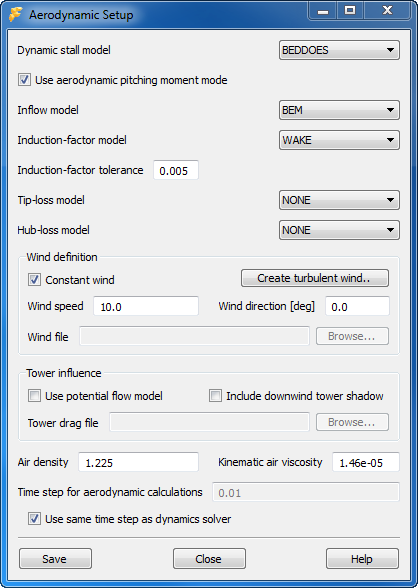
\includegraphics[width=0.6\textwidth]{Figures/3b-AerodynamicSetup}
\end{center}

\begin{itemize}
\item{\sl Dynamic stall model} --
  Specify BEDDOES to use the Beddoes-Leishman dynamic stall model,
  or STEADY for quasi-steady airfoil characteristics.
  It is recommended to use the BEDDOES model in most situations.

\item{\sl Use aerodynamic pitching moment mode} --
  This option enables the calculation of aerodynamic pitching moment.
  The Airfoil files must then include pitching moment coefficients ({\sl CM}).

\item{\sl Inflow model} --
  This option controls the dynamic inflow model.
  Specify GDW to use a Generalized Dynamic Wake inflow model to  calculate the
  induction factor, or BEM to use the Blade Element Momentum theory with skewed
  wake and tip loss corrections.

  The direct calculation method of the GDW option is considerably faster than
  the iterative method of the BEM option, which assumes that the wake is always
  in equilibrium with the forces on a blade element.
  See Appendix E of the AeroDyn User's Guide for more information on the dynamic
  inflow method employed with the GDW option.

\item{\sl Induction-factor model} --
  This option controls the wake or induced velocity calculation.
  There are three choices, WAKE, SWIRL and NONE.
  Use SWIRL to calculate both axial and tangential induction.
  If WAKE is specified, only the axial induction will be calculated.

  If NONE is specified, the induced velocity calculation will be completely
  bypassed and all induction factors reset to zero.
  This option is available primarily to assist the debugging of new models.
  We suggest that in the first tests of a new model, ignore the wake to
  accelerate the calculations and eliminate the possibility of convergence
  problems in the induction factor iteration. A warning is generated by AeroDyn
  when NONE is used to remind the user that this is a highly unusual situation.

\item{\sl Induction-factor tolerance} --
  This is the tolerance used for convergence testing in the iterative solution
  to find the induction factor, $\alpha$, when using the GDW inflow model.
  The default value 0.005 should be used unless there are compelling reasons
  to do otherwise.

  Sometimes it is desirable to change this value to avoid convergence problems
  (with some loss of accuracy) or to speed up the calculations.
  The value represents the maximum allowed difference between two successive
  estimates of $\alpha$. That is, if the new estimate of $\alpha$ differs from
  the estimate from the previous iteration by an amount less than the tolerance,
  the solution has converged and the last value of $\alpha$ is used.

\item{\sl Tip-loss model} --
  This option controls the tip loss model (used with the BEM inflow model only).
  There are three possible choices, PRAND, GTECH and NONE.
  PRAND is the Prandtl tip loss model, GTECH is the Georgia Tech correction to
  the Prandtl model, whereas NONE turns off the tip loss correction altogether.

  The GTECH model is intended to better model the effects of the relatively
  large inflow velocities (compared to hovering rotors, for which the Prandtl
  model was developed) experienced by wind turbine rotors spacing the tip vortex
  rings farther apart in the wake.

\item{\sl Hub-loss model} --
  This option controls the hub loss model (used with the BEM inflow model only).
  There are two possible choices, PRAND, and NONE.
  PRAND invokes the Prandtl tip loss model, to be used to determine hub losses,
  whereas NONE turns off the hub loss correction altogether.
  This option is intended to model losses experienced by the rotor blade
  elements close to the rotor hub.
  Generally, these effects are of little consequence.

\item{\sl Wind definition} --
  This part of the dialog box is used to define the undisturbed wind field
  to be used in the aerodynamic load calculation.

  \begin{itemize}
  \item{\sl Constant wind} --
    Enable this toggle to specify a constant wind using the {\sl Wind speed}
    and {\sl Wind direction} fields.
    The wind direction value is the angle (in degrees) between the rotor plane
    normal (with zero shaft tilt) and the wind direction,
    see Section 7.1 in the AeroDyn User's Guide.
  \item{\sl Wind file} --
    When the {\sl Constant wind} toggle is disabled,
    you may use the \textbf{Browse...} button to select a separate input file
    describing the wind field.
    This can either be hub-height wind data file,
    or a full-field turbulent wind data file, described in Chapter 7 and 8,
    respectively, in the AeroDyn User's Guide.
  \item{\sl Create turbulent wind..} --
    Click this button to launch the Fedem TurbWind tool to create a full-field
    turbulent wind data file for the current model, see
    \protect\hyperlink{turbulent-wind-definition}
                      {\sl"Turbulent Wind Definition"} below.
    Then use the \textbf{Browse...} button to select the resulting
    turbulent wind file.
  \end{itemize}

\item{\sl Tower influence} --
  This part of the dialog box is used to set up the tower influence
  on the wind field.

  \begin{itemize}
  \item{\sl Use potential flow model} --
    Enables the use of a tower influence model based on potential flow solution
    around a cylinder, as described in the AeroDyn Theory Manual.
    This model provides the influence of the tower on the local velocity field
    at all points around the tower, including increases in wind speed around the
    sides and the cross-stream velocity component in the tower-near flow field.
  \item{\sl Include downwind tower shadow} --
    Enables the use of a tower wake (velocity deficit) model for downwind
    rotors. This toggle has no effect for upwind turbines.
  \item{\sl Tower drag file} --
    When one or both of the two tower influence toggles are enabled,
    a tower drag file must be specified.
    It lists the drag coefficient for the tower as function of the Reynold's
    number and the tower diameter.
  \end{itemize}

\item{\sl Air density} -- Specifies the ambient air density.

\item{\sl Kinematic air viscosity} -- Specifies the kinematic air viscosity.
  This value is used in AeroDyn to calculate the local element Reynold's number,
  which can be used to move between multiple tables in the airfoil files.

\item{\sl Time step for aerodynamic calculations} --
  Specifies the time step size ($dt_{\rm AD}$) used by AeroDyn.
  Since the time integration steps in the Fedem dynamics solver ($dt$) often are
  quite small, the dynamics simulation can run faster and be more immune to
  numerical stability problems if $dt_{\rm AD}$ is specified larger than $dt$,
  but still less than the time scale for the changes in aerodynamic forces.

  Typically, the aerodynamic forces should not be expected to change faster than
  the time it takes the blade to rotate $2.4^\circ$, e.g.,
  if a rotor runs at 30 rpm, it will take 0.02 seconds for the blade to move
  $3.6^\circ$ such that $dt_{\rm AD}=0.02$ will then repeat the aerodynamic
  calculations often enough to catch the true variations in the loads.
  Since the time stepping is controlled by the Fedem dynamics solver,
  the aerodynamic calculations will be repeated after a time interval that is
  at least $dt_{\rm AD}$ (but less than $dt_{\rm AD}+dt$).
  That is, the aerodynamic calculations are not necessarily repeated exactly
  at the intervals $dt_{\rm AD}$.

\item{\sl Use same time step as dynamics solver} --
  Enable this toggle to ignore the {\sl Time step for aerodynamic calculations}
  value and always use the same step size in AeroDyn as in the dynamics solver,
  i.e., $dt_{\rm AD}=dt$.
\end{itemize}

\SubSubSection{Turbulent Wind Definition}{turbulent-wind-definition}

The Turbulent Wind Definition dialog box is used to generate turbulent wind
files for Fedem Windpower. It is basically a front-end for the TurbSim tool by
NREL (\href{https://www.nrel.gov/wind/nwtc/turbsim.html}
           {nrel.gov/wind/nwtc/turbsim.html}).
Fedem Windpower sends the parameters of the wind turbine to TurbSim, such as
hub height, grid height, time step, duration, output folder, ref. height, etc.
You should adjust these fields to match your wind turbine and conditions.

The figure below illustrates the Turbulent Wind Definition dialog box:

\clearpage
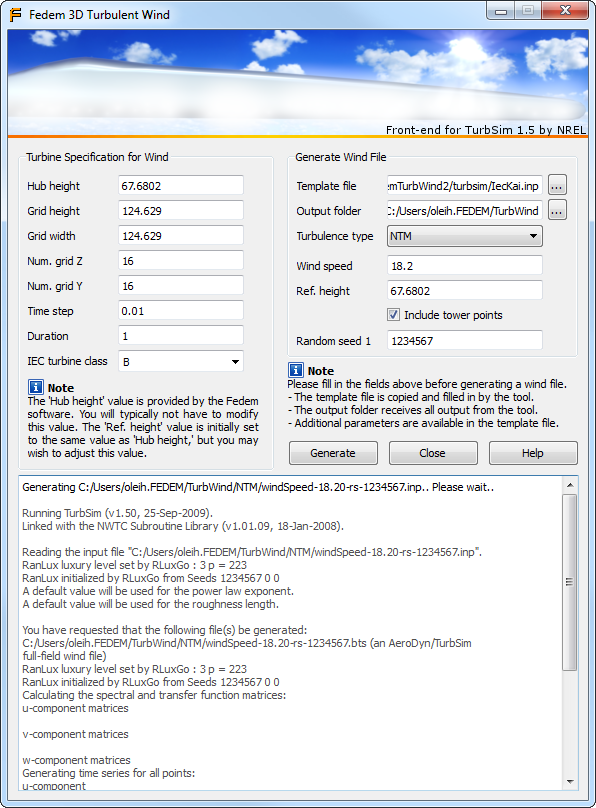
\includegraphics[width=0.85\textwidth]{Figures/3b-TurbWind}

\begin{itemize}
\item{\sl Hub height [m]} -- Specifies
  the hub height of the turbine for which the inflow is being generated. This
  parameter is used as a reference height for determining the grid location.
\item{\sl Grid height [m]} --
  This parameter is the distance between the top and bottom of the grid.
  The top of the grid is assumed to be aligned with the top of the rotor disk
  (see TurbSim User's Guide), and because all points of the grid must be above
  ground level, $0.5\times{\rm GridHeight}<{\rm HubHeight}$.
\item{\sl Grid width [m]} --
  This parameter is the width of the grid.
  The rotor is assumed to be centered horizontally on the grid.
  If you are generating FF-files for AeroDyn,
  the grid width---like the height---must be large enough to ensure that
  no part of the blade lies outside the grid, even when the system is displaced.
\item{\sl Num. grid Z} --
  Specifies the number of grid points to generate in the vertical direction.
  It must be an integer greater than 1.
\item{\sl Num. grid Y} --
  Specifies the number of grid points to generate in the horizontal direction.
  It must be an integer greater than 1.
\item{\sl Time step [s]} --
  This parameter is the time step size ($dt_{\rm TS}$).
  It is set to 0.05 seconds in the sample input files, and that value is
  recommended for most simulations. The time step determines the maximum
  frequency, $f_{\rm max}=1/t_{\rm TS}$, used in the inverse FFT-calculation.
\item{\sl Duration [s]} --
  Duration sets the analysis time and usable time in the TurbSim input file
  (see TurbSim User's Guide).
\item{\sl IEC turbine class} --
  IEC turbulence characteristic (A, B, C or TI in \%) or KHTEST.
\item{\sl Template file} --
  TurbSim input file (\File{.inp}) to use as template.
\item{\sl Output folder} --
  The folder where output files will be stored.

\item{\sl Turbulence type} --
  This parameter indicates which IEC wind model will be used.
  Valid entries, which are found in the TurbSim User's Guide,
  include the Normal Turbulence Model (NTM), Extreme Turbulence Model (ETM),
  and Extreme Wind Speed Model (EWM) using the 10-minute average wind speed
  with a recurrence period of 1 year or 50 years. Note that the
  EWM scaling parameters in TurbSim are valid only for 10-minute simulations.

  The definitions of these models and of the wind turbine classes can be found
  in the IEC 61400-1 standard (3rd edition).
  If the IEC turbine class (IECturbc) parameter was specified as a percentage
  instead of as a standard turbulence category, the wind model must be ``NTM''.
  This input is used only with the IEC spectral models.

\item{\sl Wind speed} --
  Specifies the mean stream-wise wind speed at the reference height.
  It is the mean value over the entire analysis time length of the simulation
  of the u-component wind speed.
  It must be a positive value in units of meters per second.
\item{\sl Ref. height [m]} --
  Specifies the height of the corresponding reference wind speed.
  This parameter enables users to specify the mean wind speed at a height other
  than the hub height. TurbSim uses this reference height and wind speed
  with the wind profile type to calculate the hub-height mean wind speed.
\item{\sl Include tower points} --
  Determines whether TurbSim generates binary tower time series,
  which contain points in a line at the tower centerline from the bottom
  of the rectangular grid to the ground.
\item{\sl Random seed 1} --
  This input parameter is used in conjunction with the next parameter,
  {\sl RandSeed2}, in the \File{.inp} file; it tells TurbSim how to initialize
  the {\sl pRNG} value. The random seed must be an integer in the range
  $[-2147483648,2147483647]$.

  The random numbers generated by the {\sl pRNG} are used to create random
  phases (one per frequency per grid point per wind component) for the velocity
  time series. When {\sl pRNG} is initialized in the same way
  (i.e., {\sl RandSeed1} and {\sl RandSeed2} are not changed),
  the user can reproduce the same random phases between runs,
  which is useful in comparing the effects of changes to other input parameters.
  Random numbers also are used to generate some default input values and the
  superimposed coherent structures for the non-IEC spectral models.
\end{itemize}

Click the \textbf{Generate} button to run TurbSim for generating output files
in the output folder. The console output from TurbSim is listed in
the lower text area of the dialog box.


\SubSection{Tower definition}{tower-definition}

The Tower Definition dialog box, which is shown below,
is used to create a more complex tower based on the following fields:

\begin{itemize}
\item{\sl D1 [m]} --
  Specifies the diameter of the tower at the top.
\item{\sl D2 [m]} --
  Specifies the diameter of the tower at the bottom.
\item{\sl T [m]} --
  Displays the total tower height.
\item{\sl H1 [m]} --
  Specifies the height of the lower part of the tower.
\item{\sl H2 [m]} --
  Displays the height of the upper part of the tower.
\item{\sl Wall thickness [m]} --
  Specifies the thickness of the wall.
\item{\sl Material} --
  Specifies the tower material.
\item{\sl Rho}, $E, \nu, G$ --
  Display the properties of the selected tower material.
\item{\sl N1} --
  Specifies the number of beam elements in the lower half.
\item{\sl N2} --
  Specifies the number of beam elements in the upper half.
\end{itemize}

\noindent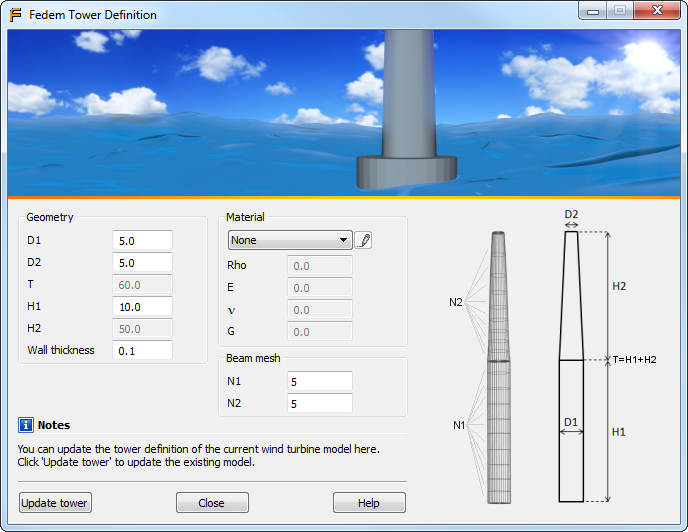
\includegraphics[width=\textwidth]{Figures/3b-TowerDefinition}

The Tower Definition dialog box is available only if the initial turbine
model was generated with a tower height larger than zero. Otherwise, the
tower (if needed), has to be added manually, by importing a separate FE
part (see \refSection{creating-parts-by-file-import}
                     {Creating parts by file import}
or a spaceframe (see
\refSection{import-of-space-frames}{Import of space frames}),
and manually attaching it to the master triad of the yaw joint (see
\refSubSection{attaching-joints}{Attaching joints}{using-the-attach-command}.


\SubSection{Control system}{control-system}

The \protect\hyperlink{turbine-definition}{\sl Turbine definition} dialog box
includes a check box for including a tailored control system with the wind
turbine model.
This control system provides the following:

\begin{itemize}
\item A low-pass filter on the generator rotation velocity.
\item A pitch controller for the z-rotation.
\item A general pitch controller.
\end{itemize}

The figures below show the properties of the control system functions:

\clearpage\noindent
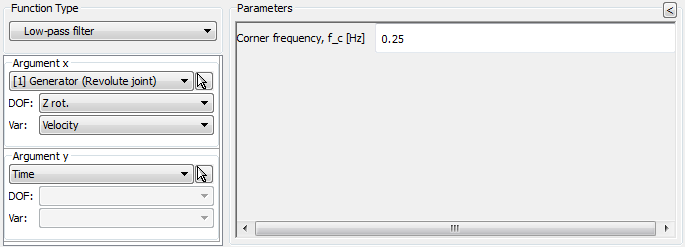
\includegraphics[width=0.98\textwidth]{Figures/3b-ControlSysFunc1}
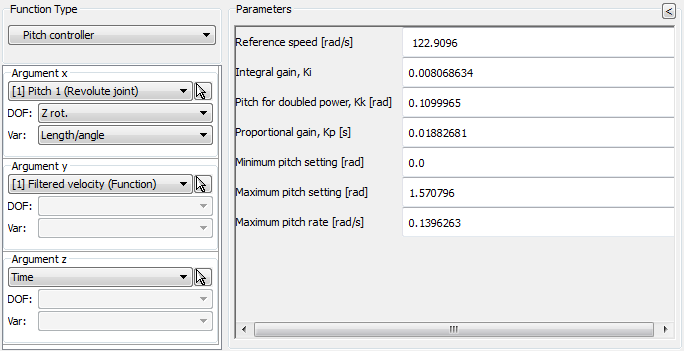
\includegraphics[width=0.98\textwidth]{Figures/3b-ControlSysFunc2}
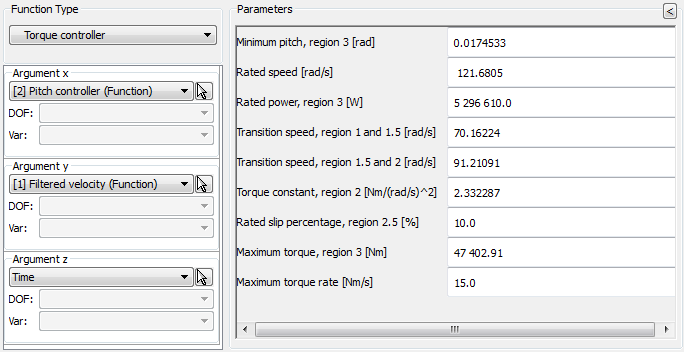
\includegraphics[width=0.98\textwidth]{Figures/3b-ControlSysFunc3}

Fedem Windpower also supports more general control system modeling.
See \refChapter{control-system-modeling}{Control System Modeling}
for more details.


%%%%%%%%%%%%%%%%%%%%%%%%%%%%%%%%%%%%%%%%%%%%%%%%%%%%%%%%%%%%%%%%%%%%%%%%%%%%%%%%
\Section{Advanced solving and analysis}{advanced-solving-and-analysis}

When the wind turbine model is completed, with proper blade definitions,
control system, load conditions, aerodynamic setup, etc., the simulation can be
started by a simple click of a button, as described in
\refSection{basic-solving-and-analysis}{Basic solving and analysis}.
However, often the model is so complex that more tuning of the simulation setup
is needed. We will describe some additional tools available in Fedem Windpower,
for the solving and analysis of wind turbine models below.


\SubSection{Running the dynamics solver (advanced mode)}
           {running-the-dynamics-solver-advanced-mode}

\begin{wrapfigure}[6]{r}{0.5\textwidth}
  \vskip-\baselineskip
  \includegraphics[trim=0 0 0 350,clip,width=0.5\textwidth]{\ReferenceImg/dlg-solver-basic1}
\end{wrapfigure}

You can display the {\sl advanced} Dynamics Solver Setup dialog box by
choosing \textbf{Dynamics Solver (Advanced Mode)...} on the {\sl Solve}
menu, or click the \textbf{Advanced} button (shown to the right) in the
lower right part of the {\sl basic} Dynamics Solver Setup dialog box,
discussed in
\refSection{running-the-dynamics-solver-basic-mode}
           {Running the dynamics solver (basic mode)}.

The advanced Dynamics Solver Setup dialog box contains several settings
where you, for instance, can adjust the time integration parameters,
nonlinear iterations, convergence tolerance settings, etc.
Refer to \refSection{dynamics-solver-advanced-mode}
                    {Dynamics Solver (Advanced Mode)}
for full details on all the options available in this dialog box.

\clearpage


\SubSection{Advanced results analysis}{advanced-results-analysis}

We will have a look at a few advanced analysis techniques here that are
useful when analysing wind turbine models.

\subsubsection{Result file browser}

When running the dynamics solver, a results database is established on disk.
The figure below illustrates the Result File browser, which is a dialog box
for viewing the contents of the results database.
See \refSection{result-file-browser}{Result File Browser}
for a general description of this dialog box. For wind turbine models,
there is an additional set of files listed here one should know about:

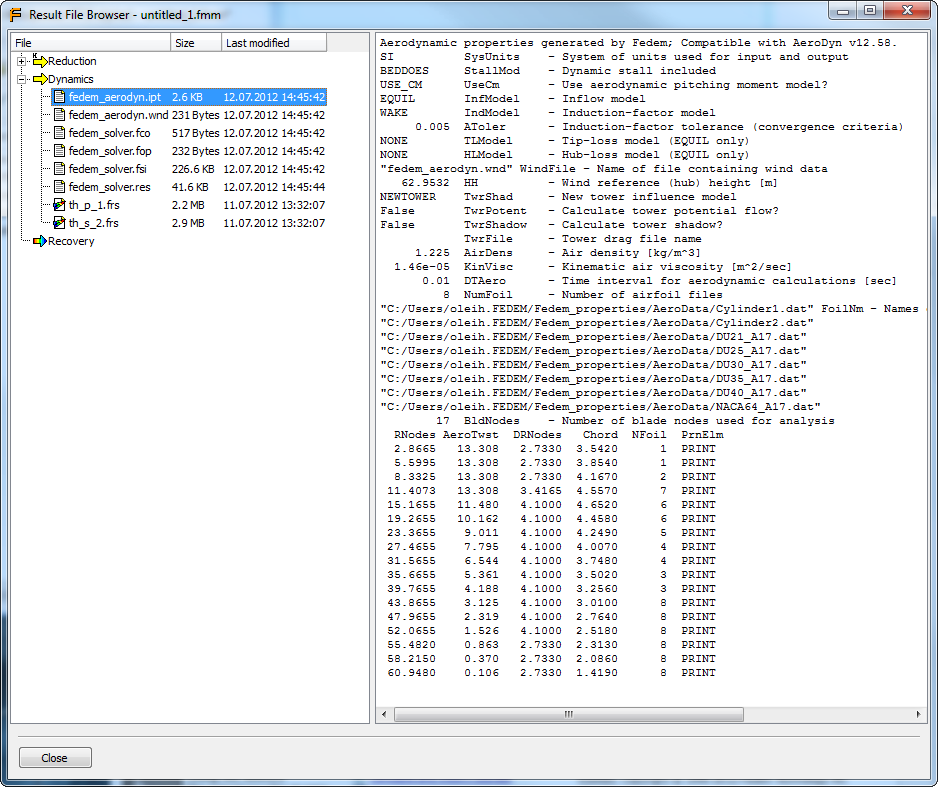
\includegraphics[width=0.95\textwidth]{Figures/3b-ResultFileBrowser}

First of all is the \File{.ipt} file, which is the main input file for AeroDyn.
The content of this file can be viewed (as shown in the figure above) by
clicking on the file name in the left part of the dialog box.
Here you can see what is sent to AeroDyn.
Next is the \File{.wnd} file, which contains the description of the wind field.
This can either be a deterministic wind, or a turbulent wind,
generated by TurbSim.

\subsubsection{Fatigue summary}

Another useful tool is fatigue summary. You can do a fatigue summary analysis
on any graph or set of curves in Fedem Windpower.
Just select a graph or set of curves, right click them,
and choose \textbf{Fatigue Summary...}.
If you have multiple events in your model, then fatigue summary will be
calculated for each event. You can adjust the probability values ({\sl Prob}).

\noindent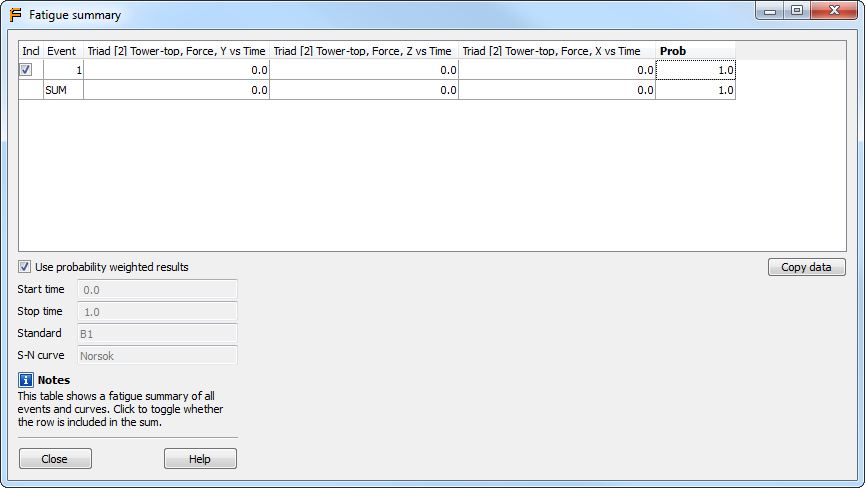
\includegraphics[width=\textwidth]{Figures/3b-GraphsMEF}
